\DiaryEntry{Division Theorem, Least Common Multiple, and $ax + by = c$}{2020-08-11}{Category}

\subsection{Division Algorithm}

\begin{theorem}
  Given two integers $a,b$ with $b > 0$, there exist unique integeers $q, r$ satisfying

  \bee
  a = qb + r, \quad 0 \leq r < b
  \eee

  The integer $q$ is called the quotient, the integer $r$ is called the remainder.
\end{theorem}

Intuitively, the theorem is true: The product $qb$ can take on the values $b, 2b, 3b, \dots$ and the value $a$ sits somewhere ``in between''. Since the remainder has to be positive, $q = \lfloor \frac{a}{b} \rfloor$ and the remainder $r$ ``fills up'' the space between $q$ and $a$. If we restrict $r$ to $0 \leq r < b$, then $r,q$ are unique: If $a = qb$, then nothing needs to be filled up, therefore $r = 0$. On the other hand, the largest value for $r$ is when $a = (q+1)b-1$ with $r = b-1$.

This is shown in the following Figure.

\begin{figure}[H]
\centering
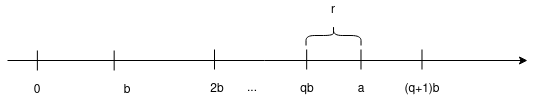
\includegraphics[scale=0.7]{images/division_stuff_1.png}
\end{figure}

\qed

Had we allowed a larger range of $r$; e.g. $0 \leq r < 2b$, there would be two choices for $r$ and $q$: The one from above with $q = \lfloor \frac{a}{b}\rfloor$ and $r = a - qb$ and the second one with $q = \lfloor \frac{a}{b}\rfloor - 1$; i.e. ``one to the left'' and $r = a - qb = a - \lfloor \frac{a}{b}\rfloor b + b$.

The theorem extends naturally to negative values of $b$; in this case

\bee
a = qb + r, \quad 0 \leq r < |b|
\eee

We can use this theorem to show various facts about divisibility of numbers.

\paragraph{Divisibility by $4$.} We first note that a number $n$ is either even or odd; this can be represented as $n = 2q$ and $n = 2q+1$, respectively. The square of the number is then either $4q^2$ or $4q^2 + 4q + 1 = 4(q^2+q) + 1$. From this we can deduce that a squared number is divisible by $4$ with zero remainder or remainder $1$. \qed

As an example, $25 / 4 = 6 \cdot 4 + 1, 36 / 4 = 9 \cdot 4$.

\paragraph{Square of odd Integers.} The square of an odd integer is of the form $8k+1$. We start by representing integers by one of the four forms $4k, 4k+1, 4k+2, 4k+3$. Since $4k$ is even (no matter if $q$ is even or odd), only $4k+1$ and $4k+3$ are odd. Squaring them yields

\bee
(4k+1)^2 = 16k^2 + 8k + 1 = 8(2k^2+k) + 1 = 8 q + 1
\eee

and

\bee
(4k+3)^2 = 16k^2 + 24k + 9 = 8(2k^2 + 3k+1) + 1 = 8q + 1 \qed
\eee

\paragraph{$N = \frac{a(a^2+2)}{3}$ is an Integer.} Same story; we express our integer as one of $3k, 3k+1, 3k+2$. Inserting these three options into the expression yields

\bee
N = \frac{3k(9k^2+2)}{3} = k(9k^2+2),
\eee

and

\bee
N = \frac{(3k+1)((3k+1)^2+2)}{3} = \frac{27k^3 + 27k^2 + 15k+3}{3} = 9k^3 + 9k^2 + 5k + 1,
\eee

and

\bee
N = \frac{(3k+2)((3k+2)^2+2)}{3} = \frac{27k^3 + 54k^2 + 42k+12}{3} = 9k^3 + 18k^2 + 14k + 4.
\eee

It can be seen that all three options yield integer values. \qed

\subsection{Least Common Multiple}

There are three entries related to the GCD: \href{2017-04-26:entry}{this one}, \href{2017-05-01:entry}{this one}, and \href{2017-09-28:entry}{this one}.

Closely related to the GCD is the least common multiple (LCM) of two numbers. An integer $c$ is a \emph{common multiple} of two nonzero integers $a, b$, if $a | c$ and $b | c$. The set of common multiples contains a smallest integer and that's the LCM. The formal definition is as follows.

The LCM $m = \lcm(a,b)$ of two nonzero integers $a, b$ is defined as
\begin{itemize}
\item $a|m$ and $b|m$.
\item If $a|c$ and $b|c$ , with $c > 0$, then $m \leq c$.
\end{itemize}

The following theorem yields a practical way to calculate the LCM.

\begin{theorem}
  For positive integers $a, b$, we have
  \bee
  \gcd(a,b)\lcm(a,b) = ab
  \eee
\end{theorem}

\begin{proof}
  We use $d = \gcd(a,b)$ and write $a = dr, b = ds$ for some integers $r,s$. We further define $m = ab / d$, then $m = dr b / d = rb$ and also $m = a ds / d = as$. Therefore $m$ is is positive common multiple of $a$ and $b$. We want to show that $m$ is the smallest common multiple.

  Now let $c$ be any common multiple of $a$ and $b$; we use $c = au = bv$. From the GCD entries, we know that thee exist integhers $x, y$ such that $\gcd(a,b) = d = ax + by$. Therefore we have

  \bee
  \frac{c}{m} = \frac{cd}{ab} = \frac{c(ax + by)}{ab} = \frac{c}{b}x + \frac{c}{a}y = vx + uy
  \eee

  From this equation we conclude that $c$ is a multiple of $m$; i.e. $m | c$ and therefore $m \leq c$. From the above LCM definition, therefore $m = \lcm(a,b)$, that is

  \bee
  \lcm(a,b) = \frac{ab}{\gcd(a,b)}
  \eee
\end{proof}

The GCD can take on values in the range of $1$ (if $a$ and $b$ are coprime) up to $\min(a,b)$ (when $a$ is a multiple of $b$ or vice versa). Therefore, the LCM can take on values in the range of $\max(a,b)$ (when $a$ is a multiple of $b$ or vice versa) to $ab$ (when $a$ and $b$ are coprime).

\subsection{The Diophantine Equation $ax + by = c$}




%%% Local Variables:
%%% mode: latex
%%% TeX-master: "journal"
%%% End:
